\begin{figure}[htb!]
	\centering
	\footnotesize

	\psfrag{a}[c][c] {$5$}
	\psfrag{b}[c][c] {$1$}
	\psfrag{c}[c][c] {$2$}

	\psfrag{d}[c][c] {$0$}
	\psfrag{e}[c][c] {$-1$}
	\psfrag{f}[c][c] {$0$}

	\psfrag{g}[c][c] {$0$}
	\psfrag{h}[c][c] {$1$}
	\psfrag{i}[c][c] {$6$}

	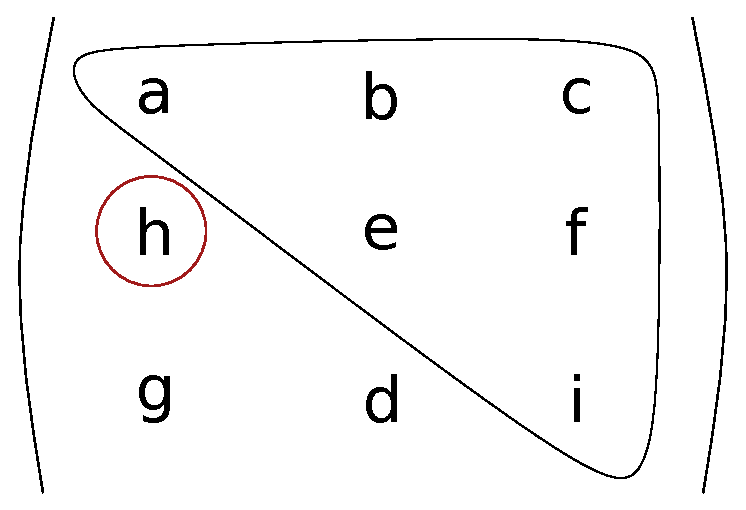
\includegraphics[width=0.4\textwidth]{matrixA21.eps}
	\caption{The entry $A_{21}$ of matrix $A$ is the only one that we may clean up
		so as to obtain a right upper triangular matrix. Givens-Rotation matrix is $G_{21}$.}
	\label{\LABEL}
\end{figure}
